\section{Auswertung}
\label{sec:Auswertung}
Um die molare Wärmekapazität aus Gleichung \ref{eqn:cmol} zu bestimmen, muss die zugeführte
Wärmemenge ermittelt werden. Diese lässt sich mit den gemessenen Strom-Spannungs-Messwerten über
die Formel
\begin{equation}
  \Delta Q = UI\Delta t
  \label{eqn:zuführ}
\end{equation}
berechnen.
Somit folgt aus Formel \ref{eqn:cmol} und \ref{eqn:zuführ} und einer Stoffmenge $n=\sfrac{m}{M}$
für die Molwärme bei konstantem Druck der Ausdruck
\begin{equation}
  C_p=\frac{UIM\Delta t}{\Delta T m}.
  \label{eqn:Cp}
\end{equation}
Die Masse $m$ der Probe ist mit $m=\SI{0.342}{\kg}$ gegeben und die molare Masse $M$ von
Kupfer beträgt $\SI{63.55}{\g\per\mol}$ \cite{kompress}.
Um die Temperatur zu berechnen wird die monotone Temperaturfunktion der
Pt-100-Widerstände verwendet, welche in Gleichung \ref{eqn:Widerstand}
%\begin{equation}
%  T=0,00134R^2 + 2,296R - 243,02
%  \label{eqn:Pt100}
%\end{equation}
gegeben ist. %Dabei bezeichnet $R$ den Widerstand in Ohm.
Die Messwerte, als auch die berechneten Werte der Probentemperatur und die
Molwärme bei konstantem Druck sind in Tabelle \ref{tab:tab1} angegeben.\\
\\
Als Fehler für die Messgräte (Ampere-, Volt- und Ohm-Meter) wird ein Fehler von
$\pm 1$ auf die erste Nachkommastelle angenommen. Für die Ablesezeit wird ein
Fehler von 3\;s angenommen.
Dabei werden die Fehler mit der Gauß´schen Fehlerfortpflanzung:
\begin{equation}
  \increment f = \sqrt{ \sum_{i=1}^N \left( \frac{\partial f}{\partial x_i}\right)^2
  \cdot (\increment x_i)^2  } \:
  \label{eqn:gaus}
\end{equation}
berechnet. Für $C_P$ ergibt sich:
\begin{equation}
  \Delta C_P=\sqrt{\Big(\frac{I\Delta t M}{\Delta T m}\Big)^2 (\Delta U)^2+\Big(\frac{U\Delta t M}{\Delta T m}\Big)^2 (\Delta I)^2
  +\Big(\frac{UIM}{\Delta m}\Big)^2 (\Delta t)^2  +\Big (-\frac{UI\Delta t M}{m \Delta T^2}\Big)^2 (\Delta T)^2}.
  \label{eqn:fehler}
\end{equation}
\begin{table}[H]
  \centering
  \caption{Messwerte der Wärmepumpe}
  \label{tab:tabe1}
    \begin{tabular}{S S S S S S}
    \toprule
    $ t  \: / \si{\second} $ & $ p_a \: / \si{\bar} $ & $ p_b \: / \si{\bar} $ &
    $ T_1 \: / \si{\kelvin} $ & $ T_2 \: / \si{\kelvin} $ & $ P \: / \: \si{\watt} $\\
    \midrule
    0 & 5.0 & 5.0 & 293.65 & 293.65 & 0 \\
    60 & 4.7 & 6.0 & 294.15 & 293.55 & 115 \\
    120 & 4.4 & 6.4 & 295.15 & 293.15 & 118 \\
    180 & 4.5 & 6.9 & 296.35 & 291.95 & 122 \\
    240 & 4.6 & 7.0 & 297.55 & 290.95 & 125 \\
    300 & 4.6 & 7.0 & 298.85 & 289.95 & 125 \\
    360 & 4.5 & 7.2 & 300.05 & 289.15 & 123 \\
    420 & 4.4 & 7.4 & 301.15 & 288.45 & 123 \\
    480 & 4.3 & 7.8 & 302.35 & 287.65 & 122 \\
    540 & 4.2 & 8.0 & 303.55 & 286.95 & 122 \\
    600 & 4.2 & 8.1 & 304.65 & 286.25 & 121 \\
    660 & 4.1 & 8.3 & 305.75 & 285.55 & 121 \\
    720 & 4.0 & 8.5 & 306.75 & 284.95 & 121 \\
    780 & 4.0 & 8.8 & 307.75 & 284.35 & 121 \\
    840 & 3.9 & 9.0 & 308.75 & 283.75 & 121 \\
    900 & 3.8 & 9.1 & 309.65 & 283.15 & 121 \\
    960 & 3.8 & 9.2 & 310.55 & 282.55 & 122 \\
    1020 & 3.8 & 9.5 & 311.45 & 282.05 & 122 \\
    1080 & 3.7 & 9.8 & 312.25 & 281.55 & 122 \\
    1140 & 3.7 & 10.0 & 313.05 & 281.15 & 122 \\
    1200 & 3.7 & 10.0 & 313.9 & 280.65 & 122 \\
    1260 & 3.6 & 10.2 & 314.65 & 280.25 & 123 \\
    1320 & 3.6 & 10.3 & 315.35 & 279.85 & 123 \\
    1380 & 3.6 & 10.6 & 316.15 & 279.45 & 124 \\
    1440 & 3.6 & 10.8 & 316.85 & 279.15 & 124 \\
    1500 & 3.6 & 11.0 & 317.55 & 278.75 & 124 \\
    1560 & 3.6 & 11.1 & 318.25 & 278.55 & 124 \\
    1620 & 3.6 & 11.2 & 318.95 & 278.25 & 125 \\
    1680 & 3.5 & 11.4 & 319.55 & 277.95 & 125 \\
    1740 & 3.5 & 11.5 & 320.15 & 277.65 & 125 \\
    1800 & 3.5 & 11.7 & 320.75 & 277.45 & 125 \\
    1860 & 3.5 & 11.9 & 321.35 & 277.25 & 125 \\
    1920 & 3.5 & 12.0 & 321.95 & 277.05 & 125 \\
    1980 & 3.5 & 12.1 & 322.45 & 276.95 & 125 \\








      \bottomrule
    \end{tabular}
\end{table}



Mittels der Korrekturformel aus Gleichung \ref{eqn:cpcv}
%\begin{equation}
%  C_p - C_V= 9\alpha^2\kappa V_0 T
%  \label{eqn:korrektur}
%\end{equation}
lässt sich die molare Wärmekapazität bei konstantem Volumen berechnen.
Der Fehler ergibt sich zu
\begin{equation}
  \Delta C_V=\sqrt{(\Delta C_p)^2 +(-9V_0 \alpha^2 \kappa)^2(\Delta T)^2 +(-9TV_02\alpha\kappa)^2(\Delta \alpha)^2}.
\end{equation}
Für das Kompressionsmodul wird der Wert $\kappa=\SI{137.8}{\giga\Pa}$ \cite{kompress}
und für das Molvolumen wird $V_0=\SI{7.11}{\cm^3\per\mol}$
\cite{mol} verwendet.

%Dabei bezeichnet
%$\kappa=\SI{137.8}{\giga\Pa}$ das Kompressionsmodul und $V_0=\SI{7.11}{\cm^3\per\mol}$
%das Molvolumen von Kupfer.
Die Werte für den linearen Ausdehnungskoeffizienten $\alpha$
werden mit Hilfe der Tabelle aus der Versuchsanleitung \cite{skript} ermittelt.
Die gegebenen Werte werden in Abbildung \ref{fig:alpha} gegen $\sfrac{1}{T}$
aufgetragen und mit der Formel
\begin{equation}
  \alpha(x)= \frac{m}{x}+b
\end{equation}
gefittet. Die Ausgleichsrechnung ergibt folgende Parameter:
\begin{align}
  m &= \SI{-872.2(38)e-6}{}\\
  b &= \SI{19.40(3)}{\per\K}.
\end{align}
\begin{figure}[H]
  \centering
  \includegraphics[height=9cm]{alpha.pdf}
  \caption{Linearer Zusammenhang des Ausdehnungskoeffizienten $\alpha$ mit der
  inversen Temperatur $\sfrac{1}{T}$.}
  \label{fig:alpha}
\end{figure}

Die Ergebnisse für $\alpha$ und $C_V$ sind in Tabelle \ref{tab:tab2} zu sehen.
\begin{table}[H]
  \centering
  \caption{Wertetabelle für $\alpha$ und $C_V$.}
  \label{tab:tab2}
    \begin{tabular}{S S S S S}
    \toprule
    $ T\: \text{in}\: \si{\K} $ & $ {\alpha \cdot 10^{-6} \: \text{in}\: \si {\per\K}} $ &
    $ C_V \: \text{in}\: \si{\J\per\K\mol} $\\
    \midrule %Cv, a *10-6, Cv
    %0 & 1 & 1\\
    88.60\pm0.24 & 9.56\pm0.06 & 14.17\pm8.13  \\ %&3.6 & 318.97\pm0.85\\
    93.81\pm0.24 & 10.10\pm0.06 & 17.58\pm10.03 \\ %& 4.7 & 440.90\pm1.11\\
    99.74\pm0.24 & 10.66\pm0.05 & 15.52\pm8.84 \\ %& 5.1 & 508.68\pm1.21\\
    104.74\pm0.24 & 11.07\pm0.05 & 18.44\pm10.52 \\ %& 4.6 & 481.79\pm1.09\\
    110.94\pm0.24 &  11.54\pm0.05 & 14.86\pm8.45 \\ %& 5.3 & 587.97\pm1.27\\
    115.96\pm0.24 & 11.89\pm0.05 & 18.49\pm10.52 \\ %& 4.6 & 533.41\pm1.10\\
    121.47\pm0.24 &  12.22\pm0.05 & 16.83\pm9.57 \\ %& 4.9 & 595.21\pm1.17\\
    126.99\pm0.24 & 12.53\pm0.04 & 16.79\pm9.54 \\ %& 4.9 & 622.29\pm1.18\\
    131.58\pm0.24 & 12.77\pm0.04 & 20.42\pm11.62 \\ %& 4.2 & 552.62\pm1.01\\
    136.65\pm0.24 & 13.02\pm0.04 & 18.40\pm10.47 \\ %& 4.6 & 628.57\pm1.11\\
    141.49\pm0.24 & 13.24\pm0.04 & 19.28\pm10.97 \\ %& 4.4 & 622.54\pm1.07\\
    146.34\pm0.24 & 13.44\pm0.04 & 19.24\pm10.95 \\ %& 4.4 & 643.88\pm1.07\\
    150.95\pm0.24 & 13.62\pm0.04 & 20.22\pm11.52 \\ %& 4.3 & 649.11\pm1.05\\
    155.34\pm0.24 & 13.79\pm0.04 & 21.31\pm12.14 \\ %& 4.1 & 636.88\pm0.98\\
    159.97\pm0.24 & 13.95\pm0.04 & 20.12\pm11.47 \\ %& 4.3 & 687.89\pm1.05\\
    164.62\pm0.24 & 14.10\pm0.04 & 20.18\pm11.51 \\ %& 4.3 & 707.87\pm1.06\\
    168.79\pm0.25 & 14.23\pm0.04 & 22.54\pm12.86 \\ %& 3.9 & 658.27\pm0.95\\
    173.45\pm0.25 &  14.37\pm0.04 & 20.08\pm11.46 \\ %& 4.3 & 745.84\pm1.06\\
    178.13\pm0.25 &  14.50\pm0.04 & 20.04\pm11.44 \\ %& 4.3 & 765.94\pm1.06\\
    182.56\pm0.25 &  14.62\pm0.04 & 21.11\pm12.06\\
    192.70\pm0.25 &  14.87\pm0.04 & 18.41\pm10.47\\
    200.15\pm0.25 &  15.04\pm0.04 & 25.19\pm14.28\\
    208.87\pm0.25 &  15.23\pm0.04 & 21.43\pm12.18\\
    217.12\pm0.25 &  15.38\pm0.04 & 22.65\pm12.88\\
    225.15\pm0.25 &  15.53\pm0.03 & 23.27\pm13.24\\
    232.70\pm0.25 &  15.70\pm0.03 & 24.75\pm14.08\\
    240.53\pm0.25 &  15.74\pm0.03 & 23.84\pm13.58\\
    248.39\pm0.25 &  15.89\pm0.03 & 23.74\pm13.53& \\
    256.01\pm0.25 &  15.97\pm0.03 & 24.46\pm13.94 \\
    263.41\pm0.26 &  16.01\pm0.03 & 25.22\pm14.38 \\
    271.08\pm0.26 &  16.18\pm0.03 & 24.26\pm13.86 \\
    278.52\pm0.26 &  16.27\pm0.03 & 25.03\pm14.29&\\
    285.98\pm0.26 &  16.35\pm0.03 & 24.92\pm14.25 \\
    293.21\pm0.26 &  16.42\pm0.03 & 25.74\pm14.72 \\
    300.98\pm0.26 &  16.50\pm0.03 & 23.87\pm13.68 \\
    308.51\pm0.26 &  16.57\pm0.03 & 24.63\pm14.12\\



      \bottomrule
    \end{tabular}
\end{table}


Der Zusammenhang zwischen der Temperatur $T$ und der Molwärme bei konstantem Volumen
$C_V$ ist in Abbildung \ref{fig:Cv} dargestellt.

\begin{figure}[H]
  \centering
  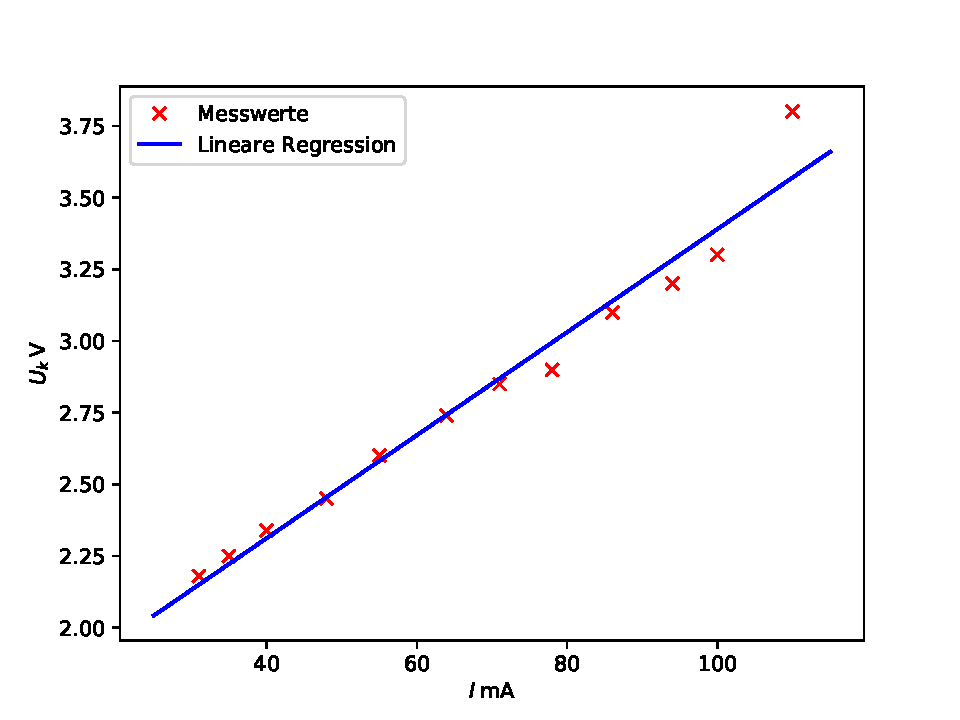
\includegraphics[height=9cm]{plot2.pdf}
  \caption{Zusammenhang zwischen der Temperatur $T$ und der Molwärme bei konstantem Volumen
  $C_V$.}
  \label{fig:Cv}
\end{figure}

Um aus den gemessenen $(C_V, T)$-Wertepaaren die Debye-Temperatur $\theta_D$ zu ermitteln
wird Tabelle 1 aus dem Skript \cite{skript} verwendet. Zunächst wird $\sfrac{\theta_D}{T}$\;
abgelesen, nach Multiplikation mit $T$ erhält man die gesuchte Debye-Tempetatur $\theta_D$.
Hier werden nur Messwerte bis $\SI{170}{\K}$ verwendet.
\begin{table}
  \centering
  \caption{Messwerte für den ersten Doppelspalt.}
   \begin{tabular}{S S| S S | S S}
    \toprule
    $x/\; \si{\mm}$& $A/\;\si{\nA}$ &
    $x/\; \si{\mm}$& $A/\;\si{\nA}$ &
    $x/\; \si{\mm}$& $A/\;\si{\nA}$ \\
    \midrule

    15.0& 4.6& 23.0& 25.0& 29.5& 6.0\\
    15.5& 4.2& 23.5& 30.0& 30.0& 5.3\\
    16.0& 4.0& 24.0& 35.0& 30.5& 4.9\\
    16.5& 4.0& 24.25& 36.0& 31.0& 4.7\\
    17.0& 4.4& 24.5& 37.0& 31.5& 4.4\\
    17.5& 5.5& 24.75& 38.0& 32.0& 4.2\\
    18.0& 6.6& 25.00& 37.0& 32.5& 3.8\\
    18.5& 7.7& 25.25& 36.0& 33.0& 3.6\\
    19.0& 8.2& 25.5& 36.0& 33.5& 3.2\\
    19.5& 8.4& 26.0& 33.0& 34.0& 3.2\\
    20.0& 8.4& 26.5& 28.5& 34.5& 3.2\\
    20.25& 8.4& 27.0& 23.0& 35.0& 3.3\\
    20.5& 8,7& 27.5& 18.0& 35.5& 3.4\\
    21.0& 9.8& 28.0& 13.5& 36.0& 3.5\\
    21.5& 12.0& 28.5& 10.0\\
    22.0& 15.0& 29.0& 7.8\\
    22.5& 20.0& 29.25& 6.7\\


   \bottomrule
  \end{tabular}
  \label{tab:tabelle3}
\end{table}

Es ergibt sich ein Mittelwert von
\begin{equation}
  \theta_{D_\text{exp}}=\SI{312.5(2)}{\K}.
\end{equation}

Der theoretische Wert für die Debye-Temperatur $\theta_{D_\text{theo}}$ wird mit der Formel
\begin{equation}
  \int_{0}^{\omega_D} Z(\omega) d\omega = 3N_L
\end{equation}
berechnet. Dabei wird die Zustandsdichte für jeden Dispersionszweig mit
\begin{align}
  Z(\omega)= \frac{V}{2\pi^2}\cdot\frac{\omega^2}{v_i^2}\:\:\:\:\text{und}\:\:\:\:
  \omega_D=\frac{k_B \theta_D}{\hbar}
\end{align}
%\begin{equation}
%  Z(\omega)= \frac{V}{2\pi^2}\cdot\frac{\omega^2}{v_i^2} \;\;\text{und}
%\end{equation}
%\begin{equation}
%  \omega_D=\frac{k_B \theta_D}{\hbar}
%\end{equation}
verwendet.
Somit ergibt sich folgender Ausdruck für die Debye-Temperatur $\theta_D$:
\begin{equation}
  \theta_D=\frac{\hbar}{k_B}\sqrt[3]{\frac{18\pi^2 N_A \rho}{M}(v_l^{-3}+2v_t^{-3})^{-1}}.
\end{equation}
%Dabei kann die Teilchenzahl mit $N_L=N_A\frac{m}{M}$ berechnet werden.
Mit den Werten $v_l=\SI{4.7}{\km\per\s}$ und $v_t=\SI{2.26}{\km\per\s}$ folgt für
den theoretischen Wert der Debye-Temperatur
\begin{equation}
  \theta_{D_\text{theo}}=\SI{331.98}{\K}.
\end{equation}
Daraus ergibt sich für die Debye-Frequenz $\omega_D$
\begin{equation}
  \omega_D=\SI{4.35e13}{\Hz}.
\end{equation}
Für die Debye-Temperatur ergibt sich aus den Werten $\theta_{D_\text{exp}}$ und $\theta_{D_\text{theo}}$
eine Abweichung von
\begin{equation}
  \frac{|\theta_{D_\text{theo}}-\theta_{D_\text{exp}}|}{\theta_{D_\text{theo}}}\cdot 100=5.9\;\%.
\end{equation}
